\documentclass[12pt]{article}
\usepackage[margin=1in]{geometry}
\usepackage{fourier}
\usepackage{graphicx}
\usepackage[import]{xypic}
\usepackage[colorlinks=true, linkcolor=blue, citecolor=blue, urlcolor=blue]{hyperref}

\newenvironment{xyoverpic}[3]
{%
\begin{xy}
\xyimport#1{\includegraphics[#2]{#3}}
}{\end{xy}}

\newenvironment{cxyoverpic}[3]
{%
\begin{center}
\centering\leavevmode\large
\begin{xyoverpic}{#1}{#2}{#3}
}{\end{xyoverpic}
\end{center}}

\setlength{\parindent}{0pt}

\begin{document}
\section{Conventions for crossings}

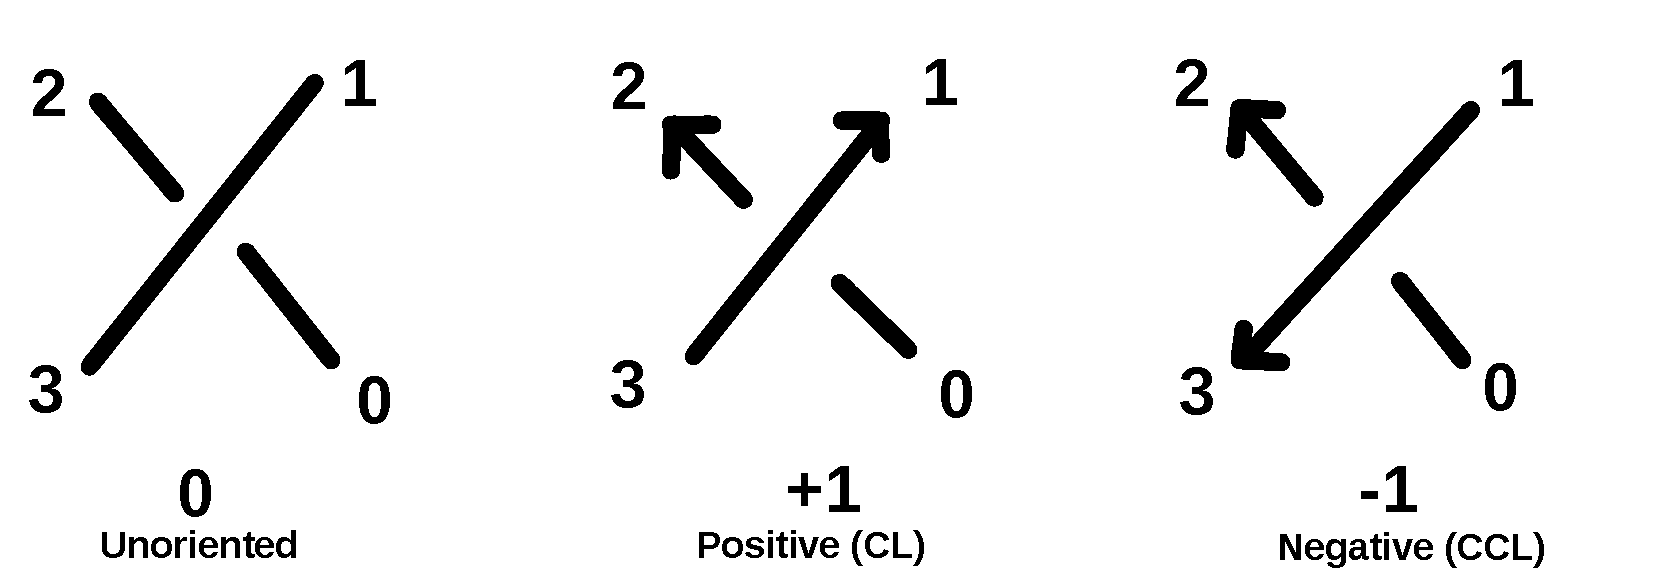
\includegraphics[scale=0.6]{pics/crossings}

\section{Conventions for tangles}

A tangle $T$ is a rectangular piece of a projection with $2n$ incoming
strands, where these strands are numbered as shown.

\begin{cxyoverpic}{(216,144)}{scale=1.0}{pics/tangle}
    ,(107,72)*{T}
    ,(39,14)*++!U{0}
    ,(64,13)*++!U{1}
    ,(84,13)*++!U{2}
    ,(156,13)*++!U{n-2}
    ,(179,13)*++!UL{n-1}
    ,(39,130)*++!DR{n}
    ,(62,131)*++!D{n+1}
    ,(155,132)*++!D{2n - 2}
    ,(178,132)*++!DL{2n - 1}
\end{cxyoverpic}


Conventions for operations and rational tangles follow

 \url{http://homepages.math.uic.edu/~kauffman/VegasAMS.pdf}

and are shown on the next page.

\pagebreak

\begin{cxyoverpic}{(432,576)}{scale=1.0}{pics/tangles}
    ,(74,439)*{T + S}
    ,(183,418)*{T \ast S}
    ,(273,484)*{\mbox{\scriptsize cross.}}
    ,(273,500)*{\mbox{\scriptsize mirror}}
    ,(270,445)*{-T}
    ,(354,440)*{\displaystyle\frac{1}{T}}
    ,(81,285)*{T \, \big\vert \, S}
    ,(231,282)*{\mbox{\normalsize Numerator closure}}
    ,(352,282)*{\mbox{\normalsize Denominator closure}}
    ,(20,235)*+!L{\mbox{\textbf{Basic rational tangles}}}
    ,(71,164)*{-2}
    ,(145,164)*{-1}
    ,(209,164)*{0}
    ,(282,164)*{1}
    ,(363,164)*{2}
    ,(69,76)*{\displaystyle -\frac{1}{2}}
    ,(152,76)*{\displaystyle-\frac{1}{1}}
    ,(212,74)*{\infty}
    ,(280,77)*{\displaystyle\frac{1}{1}}
    ,(364,74)*{\displaystyle\frac{1}{2}}
\end{cxyoverpic}




\end{document}

